\chapter{Set theory and functions}
The axiomatic formulation of set theory is pretty complicated (maybe because the concept of set is one of the most basics), therefore in this course we are only considering the intuitive idea of what a set is.

%\section{Basic concepts of set theory}

\begin{defi}[Set]
    A set is a collection of objects about which is possible to determine weather or not a particular object is a member of the set.
\end{defi}

\begin{note}
    It's worth considering also the set with no elements, the \textbf{empty set}, which is denoted by $\O$.
\end{note}

Sets are usually denoted by capital letters, and the objects within them are referred to as \textbf{elements}, which are denoted by lowercase letters.

A set can be described in two similar ways. On the one hand, the explicit way, by giving a list of their elements. One the other hand, the implicit way, by using the so called \textbf{set-builder notation}, which uses braces to enclose a property that is the qualification for membership in the set.

\begin{example}
    Let $A$ and $B$ be two sets such that
    \begin{align}
        A &= \lbrace x\st x \textrm{ is a natural number and } x^2 - 1 = 0 \rbrace = \lbrace -1, 1\rbrace \\
        B &= \lbrace x\st x \textrm{ is an even natural number } \rbrace = \lbrace x : 2\st x \textrm{ and $x$ is natural } \rbrace
    \end{align}
\end{example}

\begin{notation}
    In this previous example, both symbols $\st$ and $ : $ are used to denote \textit{such as}.
\end{notation}

We write $a\in A$ if $a$ is an element in the set $A$. Otherwise, we write $a\notin A$ to mean that $a$ is not an element in the set $A$. For instance, $2\in\N$ but $-2\not\in \N$.

\hide{For instance, 2/3 is a rational number, but not an integer one. Then
\begin{equation}
    \frac{2}{3}\in\Q,\quad\textrm{ but } \frac{2}{3}\notin\Z
\end{equation}
}

\begin{defi}[Empty set]
    We use $\O$ to refer to the set with no elements, denominated the \textbf{empty set}.
\end{defi}

\begin{defi}[Subset]
    Let $A$ and $B$ be sets. We say that $A$ is a \textbf{subset} of $B$ if every element in $A$ is an element in $B$. If $A$ is a subset of $B$ we write $A\subset B$ and we say \textit{$A$ is contained in $B$} or \textit{$B$ contains $A$}. Otherwise we write $A\notin B$.
\end{defi}

\begin{remark}
    Let $X$ be any set. Then, the empty set is a subset of $X$, $\O\subset X$.
\end{remark}

\hide{
\begin{example}
    Some examples of subsets are
    \begin{align}
        &\N\subset\Z\subset\Q\subset\R\subset\C \\
        &\O\in C\textrm{, where $C$ is any set.} \\
        &A = \{1, 2, 3\} \subset B = \{1, 2, 3, 4, 5\}
    \end{align}
\end{example}
}

\begin{defi}[Equal sets]
    Two sets $A$ and $B$ are equal if $A \subset B$ and $B\subset A$; i.e. if they have the same elements.
\end{defi}

\begin{defi}[Properly contained sets]
    We say that a set $A$ is \textbf{properly contained} in the set $B$ if $A\subset B$ but $A\neq B$.
\end{defi}

For example, $\N$ is properly contained in $\Z$ because $\N\subset\Z$, but $\N\neq\Z$.

\begin{notation}
    We use $:=$ to mean \textit{by definition}. For example, $\N := \{0, 1, 2\ldots\} $.
\end{notation}

\begin{prop}
    Let $A$ and $B$ be two sets. If $A\subset B$ and $B\subset A\implies A = B$.
\end{prop}
\begin{proof}
    Definitions of $B\subset A$ and $A\subset B$ respectively indicate that $x\in B\implies x\in A$ and that $x\in A\implies x\in B$, thus $x\in A\iff x\in B$ and therefore $A = B$.
\end{proof}

%\subsection{Power set of a set}
\begin{defi}[Power set]
    Let $A$ be a set. The power set of $A$ is a set whose elements are all the subsets of $A$, and it's denoted by $\SP\left( A \right) $.
\end{defi}

\begin{example}
    Let $A = \{a, b, c\}$, then the power set of $A$ is
    \begin{equation}
    \SP(A) = \lbrace \O, \{a\}, \{b\}, \{c\}, \{a, b\}, \{a, c\}, \{b, c\}, \{a, b, c\}\rbrace.
    \end{equation}
\end{example}

In this previous example, we must keep notice that $\O\in\SP\left( A \right)$ and $\O\subset \SP\left( A \right)$ are not exactly the same thing. In the first one we are refering to the $\O$ element in the set $\SP\left( A \right)$; while in the second, $\O$ is the empty set, which as seen previously is a subset of any set. $\{\O\}\subset \SP\left( A \right)$ has also a different meaning, as $\O$ in this case is the element contained in $\SP\left( A \right)$. We couldn't write $\{\O\}\in \SP\left( A \right)$ because the element $\{\O\}$ is not contained in $\SP\left( A \right) $.

\section{Unions and intersections of sets}
\begin{defi}[Union of sets]
    Let $A$ and $B$ be two sets. The union of $A$ and $B$ is another set whose elements are the elements in $A$ and the elements in $B$. We denote this set by $A\cup B$.
    \begin{equation}
        A\cup B \bydef \{x\st x\in A\textrm{ or } x\in B\}.
    \end{equation}
\end{defi}

\hide{
\begin{example}
    Let $A = \{a, b, c\} $ and $B = \{b, h, f\} $, then
    \begin{equation}
        A\cup B = \{a, b, c, h, f\}.
    \end{equation}
\end{example}
}

\begin{defi}[Intersection of sets]
    Let $A$ and $B$ be two sets. The intersection of $A$ and $B$ is another set whose elements are the elements that $A$ and $B$ have in common. We denote this set by $A\cap B$.
    \begin{equation}
        A\cap B  \bydef \{x\st x\in A\textrm{ and } x\in B\}
    \end{equation}
\end{defi}

\hide{
\begin{example}
    Let $A\cap B = \{b\} $ and $C = \{x, y, z\}$, then
    \begin{equation}
        A\cap C = \O \quad\rightarrow\quad\textrm{ we say that $A$ and $C$ are disjoint.}
    \end{equation}
\end{example}
}

\begin{defi}[Disjoint sets]
    Let $A$ and $B$ be two sets. If $A\cap B = \O$ it's said that $A$ and $B$ are disjoint.
\end{defi}

Let $A$, $B$ and $C$ be three non empty sets. The following properties are hold related to the union and intersection operations between those sets.
%\newpage
\bgroup
\def\arraystretch{1.5}
%\def\tabcolsep{20}
\begin{table}[h!]
\centering
\begin{tabular}{|c|c|}
    \hline
    \textbf{Property name} & \textbf{Properties} \\
    \hline
    Commutativity & $A\cap B = B\cap A$ \\
    \hline
    Commutativity & $A\cup B = B\cup A$ \\
    \hline
    Idempotency & $A\cup A = A$ \\
    \hline
    Idempotency & $A\cap A = A$ \\
    \hline
    Disjoint sets & $A\cap B = \O$ \\
    \hline
    Associativity & $\left( A\cap B \right)\cap C = A\cap\left( B\cap C \right)$ \\
    \hline
    Associativity & $\left( A\cup B \right)\cup C = A\cup\left( B\cup C \right)$ \\
    \hline
    Distributivity & $A\cup\left( B\cap C\right) = \left( A\cup B \right)\cap\left( A\cup C \right)$ \\
    \hline
    Distributivity & $A\cap\left( B\cup C\right) = \left( A\cap B \right)\cup\left( A\cap C \right)$ \\
    \hline
    Cancelation & $A\cup\left( B\cap A \right) = A$ \\
    \hline
    Cancelation & $A\cap\left( B\cup A \right) = A$ \\
    \hline
\end{tabular}
\caption{Some properties of unions and intersections of sets.}
\end{table}
\egroup

%\subsection{Venn diagrams and universal sets}
\section{Universal and complementary sets}
Sometimes it's convenient to assume that the sets that we are considering are subsets of a larger one, $\uset$, denominated the \textit{universal set}.
%Sometimes it is convenient to draw a picture of the sets we are working with. When we do this we are assuming that the sets that we are considering are subsets of some universal set which we denote by $\mathcal{U}$.

\hide{
Suppose we are considering sets $A$ and $B$. Then, we could draw the following picture, denominated \textbf{Venn diagram}.
\begin{figure}[htbp]
    \centerline{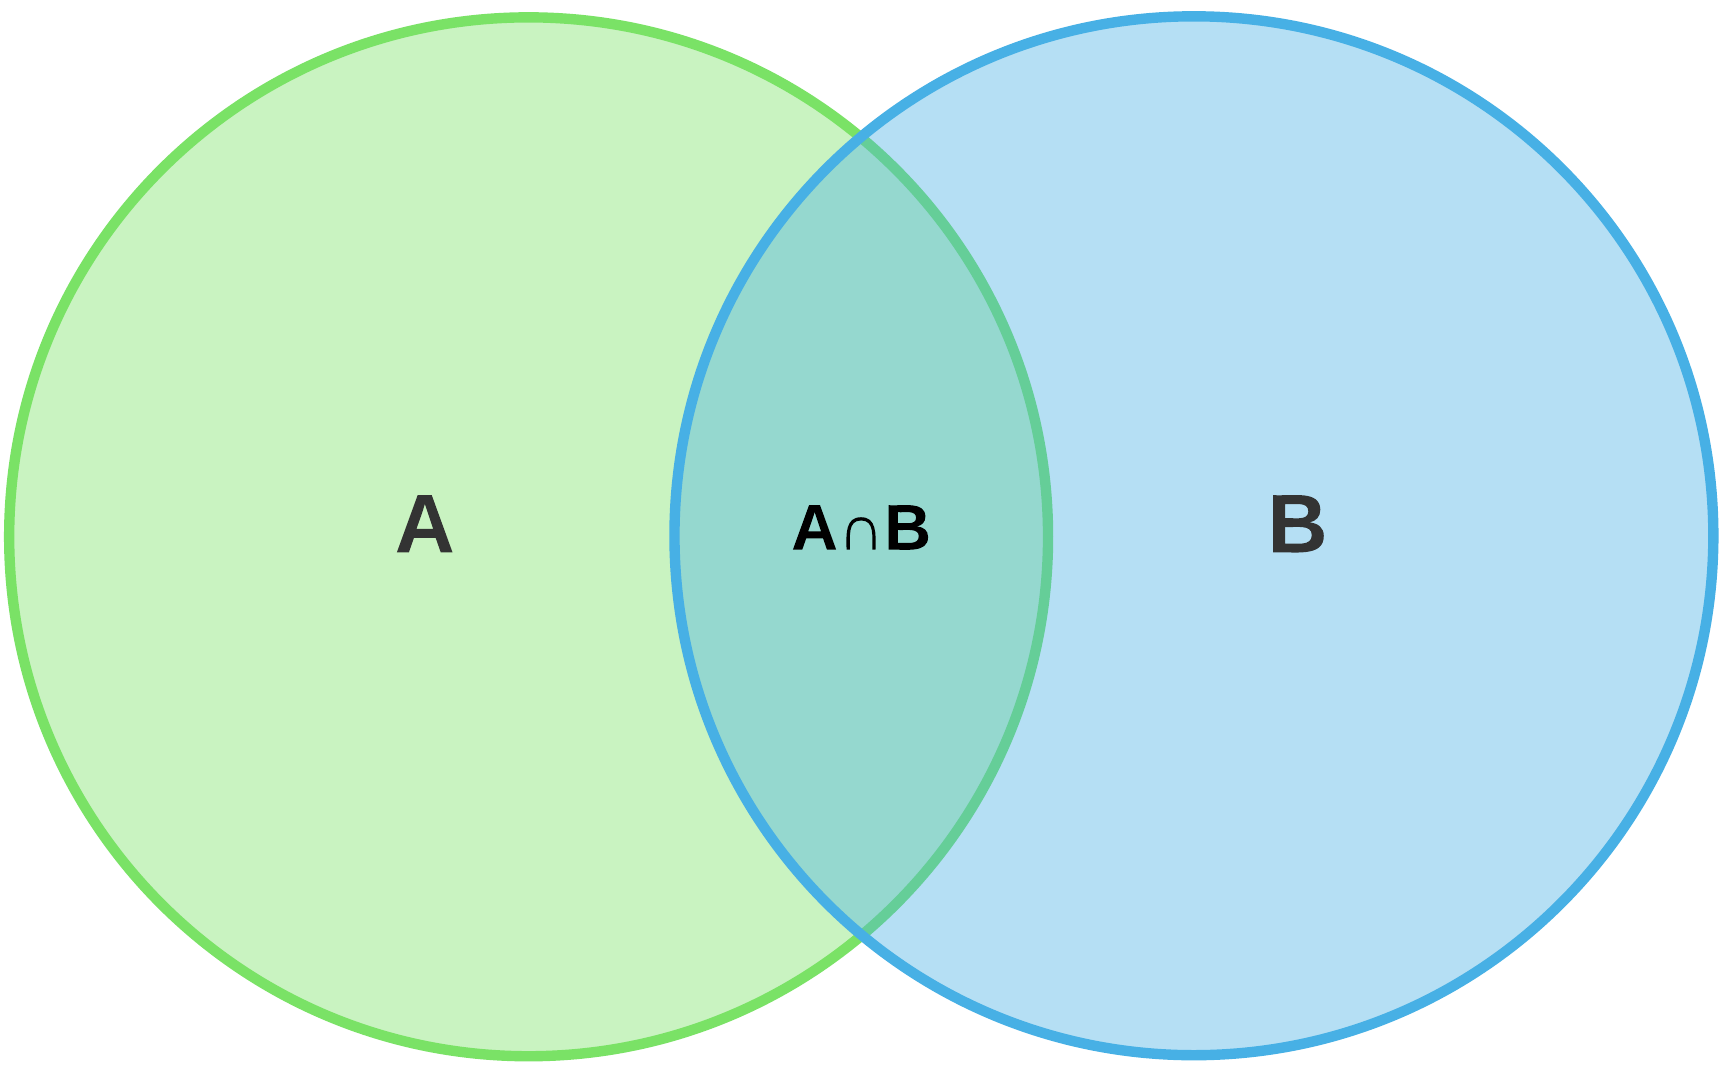
\includegraphics[width=0.4\textwidth]{venn.png}}
    \caption{Example of a Venn diagram representing the intersection of two sets $A$ and $B$.}
\end{figure}
}

\begin{remark}
    For any set $A$ we have that $A\cap\uset = A$ and $\uset\cup A = \uset$.
\end{remark}

\begin{defi}[Complement of a set]
    The complement of a set $A$ is another set such that
    \begin{equation}
        A^C = A' \bydef \{a\in\uset\st a\notin A\}.
    \end{equation}
\end{defi}

\hide{
\begin{example}
    Let $\uset = \Z$, then
    \begin{equation}
        \N\subset\uset, \quad\quad\N^C = \{x\in\Z\st x<0\}
    \end{equation}
\end{example}
}

\begin{prop}[De Morgan's laws]
et $A$ and $B$ be two sets in $\uset$. Then, the following equalities are hold.
\begin{equation}\label{demorgan:1}
    1) \left( A\cup B \right)^C = A^C\cap B^C \quad\quad\quad 2) \left( A\cap B \right)^C = A^C\cup B^C
\end{equation}

\hide{
\begin{equation}\label{demorgan:2}
    \left( A\cap B \right)^C = A^C\cup B^C
\end{equation}}
\end{prop}

\begin{proof}
    In order to prove the De Morgan's laws we need first to proof that one side of the equation is contained in the other and viceversa. Only then we can say that the equality holds.

    1) Let $x\in\left( A\cup B \right)^C \iff x\not\in A\cup B \iff x\not\in A$ and $x\not\in B \iff x\in A^C$ and $x\in B^C \iff x\in A^C\cap B^C$.
\end{proof}
    %Let $a\in\left( A\cup B \right)^C,\ a\in A^C\cap B^C$ ? So we take
    \begin{align}
        \textrm{Let } a\in\left( A\cup B \right)^C &\implies a\in\uset\textrm{ and } a\notin A\cup B \implies \\
                                     &\implies a\in\uset\textrm{ and } a\notin A\textrm{ and } a\notin B \implies \\ &\implies a\in A^C\textrm{ and } a\in B^C \implies \\
                                                         &\implies a\in A^C\cap B^C
    \end{align}
    So, we can afirm that $\left( A\cup B \right)^C \subset A^C\cap B^C $.
    \begin{align}
        \textrm{Now, let } b\in A^C\cap B^C &\implies b\in A^C\textrm{ and } b\in B^C \implies \\
                                            &\implies b\in\uset\textrm{ but } a\notin A\textrm{ and } a\notin B \implies \\ &\implies b\in\uset\textrm{ and } b\notin A\cup B \implies \\
                                            &\implies b\in \left( A\cup B \right)^C
    \end{align}
    So, we can afirm that $A^C\cap B^C\subset\left( A\cup B \right)^C $. Therefore,
    \begin{equation}
        \left( A\cup B \right)^C = A^C\cap B^C
    \end{equation}

%\end{proof}

\begin{proof}
    \textit{(Second De Morgan's law)}. In order to proof the second De Morgan's law we need first to proof that $\left( A\cap B \right)^C\subset A^C\cup B^C \textrm{ and then } A^C\cup B^C \subset \left(  A\cap B\right)^C$. Only then we can say $\left( A\cap B \right)^C = A^C\cup B^C $.
    %Let $a\in\left( A\cup B \right)^C,\ a\in A^C\cap B^C$ ? So we take
    \begin{align}
        \textrm{Let } a\in\left( A\cap B \right)^C &\implies a\in\uset\textrm{ and } a\notin A\cap B \implies \\
                                     &\implies a\in\uset\textrm{ and } a\notin A\textrm{ or } a\notin B \implies \\ &\implies a\in A^C\textrm{ or } a\in B^C \implies \\
                                                         &\implies a\in A^C\cup B^C
    \end{align}
    So, we can afirm that $\left( A\cap B \right)^C \subset A^C\cup B^C $.
    \begin{align}
        \textrm{Now, let } b\in A^C\cup B^C &\implies b\in A^C\textrm{ or } b\in B^C \implies \\
                                            &\implies b\in\uset\textrm{ but } a\notin A\textrm{ or } a\notin B \implies \\ &\implies b\in\uset\textrm{ and } b\notin A\cap B \implies \\
                                            &\implies b\in \left( A\cap B \right)^C
    \end{align}
    So, we can afirm that $A^C\cup B^C\subset\left( A\cap B \right)^C $. Therefore,
    \begin{equation}
        \left( A\cap B \right)^C = A^C\cup B^C
    \end{equation}

\end{proof}

\section{Partitions of sets}
\begin{defi}[Partition]
    A partition of a non-empty set $A$ is a separation of $A$ into mutually disjoint non-empty subsets, $A_{\alpha}$, such that $A_{\alpha}\neq A_{\beta}$ and $\cup A_{\alpha} = A$.
\end{defi}

\begin{remark}
    Note that if $A$ is a finite set then to give a partition is equivalent to writting $A$ as $A_1\cup A_2\cup\ldots\cup A_{n} $ with $A_i\neq \O$ and disjoint two by two.
\end{remark}

\hide{
\begin{example}
    Let $A = \{a, b, c, d, e\} $. A partition of $A$ could be
    \begin{equation}
        B_1 = \{a\}, \quad B_2 = \{b, e, d\}, \quad\ B_3 = \{c\}, \quad\quad B_1\cup B_2\cup B_3 = A
    \end{equation}
    \begin{equation}
        B_i\cap B_j = \O\quad\textrm{for}\quad i\neq j,\quad\quad B_i\neq\O\quad\textrm{for}\quad i = 1, 2, 3
    \end{equation}
\end{example}
}

\section{Other operations with sets}
\begin{defi}[Difference]
    Let $A$ and $B$ be two sets. The difference of $A$ and $B$ is another set, $A\textbackslash B$, whose elements are the elements in $A$ which are not contained in $B$.
    \begin{equation}
        A\textbackslash B \bydef \{a\in A \st a\notin B \}.
    \end{equation}
\end{defi}

\begin{defi}[Symmetric difference]
    Let $A$ and $B$ be two sets. The symmetric difference of $A$ and $B$ is another set, $A\triangle B$, whose elements in $A$ that are not contained in $B$ and the elements in $B$ that are not contained in $A$.
    \begin{equation}
        A\triangle B \bydef \{a\in A\st a\notin B \}\cup \{b\in B\st b\notin A \}.
    \end{equation}
\end{defi}

\begin{remark}
    $A\triangle B = A\cup B \textbackslash A\cap B$.
\end{remark}

\begin{example}
    Let $A = \{1, 2, 3, 4\} $ and $B = \{3, 5, 7\} $.
    \begin{equation}
        A\textbackslash B = \{1, 2, 4\}.
    \end{equation}
    \begin{equation}
        A\triangle B = \{1, 2, 4\}\cup \{5, 7\} = \{1, 2, 4, 5, 7\}.
    \end{equation}
\end{example}

\hide{
\begin{proposition}
    $B\triangle A = \left( A\cap B \right)^C $.
\end{proposition}
\begin{proof}
    Let $A = \{a, b, c\} $ and $B = \{c, d\} $. Consider $\uset = A\cup B$.
    \begin{align}
        B\triangle A &= \{d\}\cup \{a, b\} = \{a, b, d\} \\
        A\cap B &= \{c\} \quad\rightarrow\quad \left( A\cap B \right)^C = \{a, b, d\}
    \end{align}
    Therefore, the equality $B\triangle A = \left( A\cap B \right)^C $ is hold considering $\uset = A\cup B$.
\end{proof}
}

\begin{defi}[Cartesian product]
    Let $A$ and $B$ be two sets. The cartesian product of $A$ and $B$ is the set of the ordered pairs of the form $\left( a, b \right)$ where $a\in A$ and $b\in B$.
    \begin{equation}
        A\times B \bydef \{\left( a, b \right) \st a\in A,\ b\in B\}.
    \end{equation}
\end{defi}

\begin{example}
Let $A = \{a, b, c\} $ and $B = \{c, 3\} $.
    \begin{equation}
        A\times B = \{\left( a, c \right), \left( a, 3 \right), \left( b, c \right), \left( b, 3 \right), \left( c, c \right), \left( c, 3 \right)\}.
    \end{equation}
\end{example}

\begin{note}
    In general, $B\times A\neq A\times B$.
\end{note}

\begin{defi}[Cardinality]
    Let $A$ and $B$ be two sets. The cardinality of $A$, $\textrm{card}\left( A \right) = \abs{A}$, is the number of elements in $A$.
    \begin{equation}
        \textrm{If card}\left( A \right) < \infty\textrm{ and } \textrm{card}\left( B \right) < \infty \implies \textrm{card}\left( A\times B \right) = \textrm{ card}\left( A \right)\cdot \textrm{ card}\left( B \right).
    \end{equation}
\end{defi}

\section{Definition of function and related concepts}

\begin{defi}[Function]
    A \textbf{function}, or \textbf{map}, from a non-empty set $X$ to a non-empty set $Y$ is a subset $f$ of $X\times Y$ such that $\forall x\in X$ that appears as part of a pair in $f$, there is one, and only one $y\in Y$ such that $\left( x, y \right)\in f$, and we write $\appl{f}{X}{Y}$.
\end{defi}

In other terms, a function between two sets $X$ and $Y$ is just a way to assign an element of $X$ an element of $Y$.

\hide{
\begin{example}[An example of a function would be]
    \begin{align}
        f:\R&\to\R \quad\quad\quad\quad\quad f = \{( x, x^2 + 1)\st x\in\R \}\subset\R\times\R = \R^2 \\
        x&\to x^2 + 1
    \end{align}
\end{example}
\begin{example}
A typical non-example of a function would be
    \begin{equation}
        h\bydef\{( x,\ \pm \sqrt{x})\st x\in\R \}\subset\R\times\R = \R^2
    \end{equation}
    \begin{itemize}
        \item If $x < 0$ then $\pm\sqrt{x} \notin\R $.
        \item We would have two inputs for the very same input value:
            \begin{equation}
                (2, \sqrt{2} )\in h,\ ( 2, -\sqrt{2})\in h
            \end{equation}
    \end{itemize}
\end{example}
}

\begin{defi}
    If $\appl{f}{X}{Y}$ and $C\subset X$, $D\subset Y$, the following sets are defined.
    \begin{align}
        f\left( C \right) &= \{y\in Y\st y = f\left( x \right) \textrm{ for some } x\in C\} \\
        f^{-1}\left( D \right) &= \{x\in X\st f\left( x \right) \in D\}.
    \end{align}
\end{defi}

\hide{
\begin{definition}
    If $f:X\to Y$, the set $X$ is called the \textbf{domain} of $f$, $Y$ is the \textbf{codomain} of $f$ and $f\left( X \right) $ is the \textbf{image} (or \textrm{range}) of $f$.
\end{definition}
}

\begin{defi}
    Let $\appl{f}{X}{Y}$ and let $\appl{g}{X}{Y}$ be two functions. We say that $f = g$ if $\forall x\in X,\ f\left( x \right) = g\left( x \right)$.
\end{defi}

%\subsection{Domain, codomain and range of a function}
\begin{defi}[Domain]
    If $\appl{f}{X}{Y}$, the set $X$ is the \textbf{domain} of the function, which contains all the input values of the function.
\end{defi}

\begin{remark}
    Since a function is defined on its entire domain, its domain coincides with its domain of definition.
\end{remark}

\begin{defi}[Codomain]
    If $\appl{f}{X}{Y}$, the set $Y$ is the \textbf{codomain} of the function, which contains all of the output values of the function.
\end{defi}

\begin{defi}[Image]
    If $\appl{f}{X}{Y}$, the \textbf{image} (or \textbf{range}) of $f$ is the subset range$\subset Y$ such that
    \begin{equation}
        \textrm{range }:= \{y\in Y\st \exists,\ x\in X\textrm{ with } f\left( x \right) = y\}.
    \end{equation}
\end{defi}

\begin{notation}
    The range of a function $f$ is often denoted by $f\left( A \right) $ or by Im$f$, which stands for \textit{image of $f$}.
\end{notation}

%\subsection{Image and inverse image}
%The word \textit{image} is used in three related ways. In these definitions, $f:X\to Y$ is a function from the set $X$ to the set $Y$.
\begin{defi}[Image of an element]
    If $x\in X$, then the image of $x$ under $f$, denoted $f\left( x \right) $, is the value of $f$ when applied to $x$.
\end{defi}

\begin{note}
    $f\left( x \right) $ is alternatively known as the output of $f$ for argument $x$.
\end{note}

\begin{defi}[Image of a subset]
    The image of a subset $S\subset X$ under $f$, denoted $f\left( S \right) $, is the subset of $Y$ such that
    \begin{equation}
        f\left( S \right) \bydef \{f\left( s \right) \st x\in S\}.
    \end{equation}
\end{defi}

\begin{defi}[Image of a function]
    The \textbf{image} of a function is the image of its entire domain, also known as the range of the function.
\end{defi}

\hide{
\begin{definition}
    \textbf{(Image).} Let $f:X\to Y$ be a function and let $S\subset X$ be a subset. Then,
    \begin{equation}
        f\left( S \right):=\{y\in Y\st \exists\ s\in S\textrm{ with } f\left( s \right) = y \}
    \end{equation}
\end{definition}
}

\section{Surjective, injective and bijective functions}
\begin{defi}[Surjective function]
    A function $f$ from a set $X$ to a set $Y$ is \textbf{surjective} (also known as \textbf{onto}), if for every element $y$ in the codomain $Y$ of $f$, there is at least one element $x$ in the domain $X$ of $f$ such that $f\left( x \right) = y$. In other words, a surjective function is a function whose image is equal to its codomain. Symbolically,
    \begin{equation}
        \textrm{If } f:X\to Y\textrm{, then $f$ is said to be surjective if } \forall\ y\in Y,\ \exists\ x\in X \st f\left( x \right) = y.
    \end{equation}
\end{defi}

\begin{remark}
    It's not required that $x$ be unique; the function $f$ may map one or more elements of $X$ to the same element of $Y$.
\end{remark}

\begin{note}
    The French word \textit{sur} means \textit{over} or \textit{above}, and relates to the fact that the image of the domain of a surjective function completely covers the function's codomain.
\end{note}

\begin{notation}
    If $\appl{f}{X}{Y}$ is such that $f\left( x \right) = y$ we say that $y$ is the image of $x$ by $f$ and we'll say that $x$ is the preimage of $y$ by $f$.
\end{notation}

\begin{figure}[htbp]
    \centerline{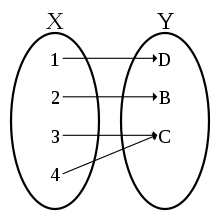
\includegraphics[width=0.25\textwidth]{surjective-function.png}}
    \caption{A surjective function from domain $X$ to codomain $Y$.}
\end{figure}

\begin{defi}[Injective function]
    Let $f$ be a function whose domain is a set $X$. The function $f$ is said to be \textbf{injective} (or \textbf{one-to-one}), provided that for all $a$ and $b$ in $X$, whenever $f\left( a \right) = f\left( b \right)$, then $a = b$. Symbolically,
    \begin{equation}
        \textrm{If } \appl{f}{X}{Y}\textrm{, then $f$ is injective if }\forall\ a, b\in X,\ f\left( a \right) = f\left( b \right) \implies a = b.
    \end{equation}
\end{defi}

\begin{figure}[htbp]
    \centering
    \begin{subfigure}{.25\textwidth}
        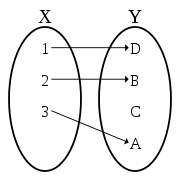
\includegraphics[width=\textwidth]{injective-nonsurjective-func.png}
        %\caption{An injective non-surjective function.}
    \end{subfigure}
    \hspace{1cm}
    \begin{subfigure}{.25\textwidth}
        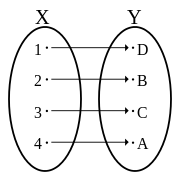
\includegraphics[width=\textwidth]{injective-surjective-func.png}
        %\caption{An injective surjective function.}
    \end{subfigure}
    %\centerline{\includegraphics[width=0.3\textwidth]{injective-function.png}}
    \caption{Injective non-surjective function (left) / Injective surjective function (right).}
\end{figure}

\begin{defi}[Bijective function]
    Let $f$ be a function from a set $X$ to a set $Y$. The function $f$ is said to be \textbf{bijective} if it's both surjective and injective. In other words, each element of one set is paired with exactly one element of the other set, and each element of the other set is paired with exactly one element of the first set.
\end{defi}

\begin{remark}
    If $X$ and $Y$ are finite sets, then the existence of a bijection means they have the same number of elements.
\end{remark}

\begin{figure}[htbp]
    \centerline{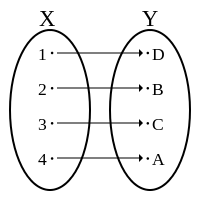
\includegraphics[width=0.25\textwidth]{bijective-func.png}}
    \caption{A bijective function, $\appl{f}{X}{Y}$.}
\end{figure}

A bijective function from the set $X$ to the set $Y$ has an \textbf{inverse function} from $Y$ to $X$.

Following these definitions, a function $\appl{f}{X}{Y}$ is surjective if and only if all the elements of $X$ are map to an element of $Y$, and it's injective if two different elements of $X$ are always applied on two different elements of $Y$; thus if we want to prove that certain $f$ is not surjective we should find an element of $Y$ that is not in the image of $f$, and if we want to prove that is not injective we should find two different elements of $X$ whose images by $f$ are the same.

\section{Composition of functions}
\begin{defi}[Composite function]
    Let $\appl{f}{X}{Y}$ and $\appl{g}{Y}{Z}$, then we define the \textbf{composition} of $g$ and $f$ as the function $\appl{g\circ f}{X}{Z}$ such that $\left( g\circ f \right) \left( x \right) = g\left( f\left( x \right)  \right) $.
\end{defi}

\begin{defi}[Identity function]
    The function $\appl{f}{X}{X}$ that leaves all of the elements invariant, this is $f\left( x \right) = x,\ \forall x\in X$, is called \textbf{identity function}, and is usually denoted by Id$_X$.
\end{defi}

\begin{defi}[Inverse function]
    Given $\appl{f}{X}{Y}$, it's said that the function $\appl{g}{Y}{X}$ is the \textbf{inverse} of $f$, denoted by $g = f^{-1}$, if $g\circ f = \textrm{ Id}_X$ and $f\circ g = \textrm{ Id}_Y$.
\end{defi}

Note that in the previous definition it's not enough to prove one condition for the other to automatically hold. For instance, if $\appl{f}{X}{\R}$ and $\appl{g}{\R}{X}$ where $X = \{x\in\R\st x \geq 0\} $ are given by $g\left( x \right) = x^2$ and $f\left( x \right) = +\sqrt{x}$, $\left( g\circ f \right) \left( x \right) = \left( +\sqrt{x}  \right)^2 = x$ holds $\forall x\in X$. However, $\left( f\circ g \right)\left( x \right) = x,\ \forall x\in X$ is not hold as negative numbers don't hold $+\sqrt{x^2} = x $.

Intuitively, the inverse of a function from $X$ to $Y$ is simply considering it on the opposite way, from $Y$ to $X$. Thsi requires every element of $Y$ to have exactly one preimage; i.e. the function must be injective.

\begin{prop}
    A function $\appl{f}{X}{Y}$ is invertible if and only if $f$ is bijective. In addition, $\left( f^{-1} \right)^{-1} = f $.
\end{prop}

\begin{prop}
    If a function $f$ is invertible, then it's inverse, $f^{-1}$, is unique, which means that there's exactly one function $f^{-1}$ satisfying this property.
\end{prop}

\begin{example}
    Let $\appl{f}{\Q}{\Q}$, $f\left( x \right) = 2x$ be a bijective function. To compute it's inverse suppose $x = f^{-1}\left( y \right) $, then $f\left( f^{-1}\left( y \right)  \right) = 2f^{-1}\left( y \right) $, and therefore $f^{-1}\left( y \right) = \frac{y}{2}$.
\end{example}

\begin{remark}
    It's easy to notice that the process to compute the inverse of $y = f\left( x \right) $ is reduced to solving for $y$ in $x = f\left( y \right) $, getting $y = f^{-1}\left( x \right) $.
\end{remark}

\hide{
\begin{definition}
    \textbf{(Inverse function).} Let $f$ be a function whose domain is the set $X$, and whose codomain is the set $Y$. Then, $f$ is \textbf{invertible} if there exists a function $g$ with domain $Y$ and image $X$, with the property
    \begin{equation}
        f\left( x \right) = y \iff g\left( y \right) = x
    \end{equation}
\end{definition}

If $f$ is invertible, then the function $g$ is unique, which means that there is exactly one function $g$ satisfying this property. That function $g$ is then called the \textbf{inverse} of $f$, usually denoted as $f^{-1}$.
\begin{proposition}
    If $f$ is an invertible function with domain $X$ and range $Y$, then
    \begin{equation}
        f^{-1}\left( f\left( x \right)  \right) = x,\quad \forall\ x\in X.
    \end{equation}
\end{proposition}
\begin{example}[.]
    Let $g:\R\to\R$ be a bijective function which $x\mapsto 2x + 1$. In order to calculate the inverse $g^{-1}:\R\to\R$ of the bijective function $g$ we should write the function in terms of $y$ and then change $y$ for $x$.
    \begin{equation}
        2x + 1 = y \quad\iff\quad x = \frac{y - 1}{2} \quad\rightarrow\quad g^{-1} = y = \frac{x - 1}{2}
    \end{equation}
    \begin{align}
        g^{-1}:\R&\to\R \\ x&\mapsto \frac{x - 1}{2}
    \end{align}
\end{example}
}
